% The technical aspects have been described very well and a very good understanding is demonstrated. A level of formality has been applied (via accepted design principles, for example) allowing for a concise but thorough description
\chapter{Design and Implementation}
\label{cha:design}
\section{Toolchain}
To develop code for the Hifive1, it was required to develop an effective method of compiling and loading code onto the board, as well as an effective debugger. Initially I used the Sifive's Freedom E SDK with PlatformIO to perform basic prototypes and experiments with the board. However these tools did not provide a sufficient level of control over what was compiled and loaded, as the SDK interacts with many parts of system that were needed for the project, as well as altering the configuration of the board. This meant that the SDK was effective for developing simple applications with the board but did not allow for low level control of operations like interrupts or privilege levels. Inspection of source code of these lead to useful insights.\\
% https://github.com/riscv-collab/riscv-gnu-toolchain reference?
To replace these tools, I used as and ld from the riscv-gnu-toolchain to assemble and link my code into an elf file that could be loaded onto the board. Also used from that collection was objdump, which was used as a disassembler. The assembler's target architecture was rv32ima\_zicsr\_zifencei, to include all the extensions available on the Hifive1, except for the compressed extension. This was done to prevent the assembler generating a mix of 32 and 16 bit operations, as this causes operations to not be word aligned, and allows jump tables to be implemented without inspecting what instructions are used. Two linker configurations were used throughout the project, the first which put both the text section and the data section into RAM, whereas the second put text and read-only data in ROM, and left the RAM free. The first configuration was used earlier, as it allowed for safe experimentation with the board while maintaining Sifive's double-tap bootloader. The double-tap bootloader allows normal operation on a regular reset but allows the board to be loaded into a safe mode when the reset is `double tapped', which loads the board into a safe and known state, so that if the board becomes otherwise inoperable it is still able to be recovered. While this was a useful feature, it limited development, as it also performed several unwanted functions, such as changing the clock configuration, and the uart configuration, which was not acceptable. The second linker config replaced the bootloader in the flash memory with the project code. This was also necessary as it was not practical to store code in RAM, as it was incredibly limited in space, so the RAM was reserved for program data.\\
To load, run and debug code on the board, I used openocd and gdb. Openocd was used to create an interface with the board, and to specify how the board should be initialized and loaded, and gdb was used to target the openocd interface, which allowed it to load elf files onto the board, and to run/debug code as normal, with some limits such as a limit to the number of breakpoints.
\section{Board Boot and Configuration}
On power on the Hifive1 will begin execution at the reset vector of 0x1004, which in this implementation is not configurable and will jump to the Mask ROM at 0x1\_0000, in which similarly cannot be configured in the Hifive1's implementation of the E31. The mask ROM will immediately jump to the \ac{otp} memory. This is configurable, but will not be done in this project. This is because the \ac{otp} memory can only be edited by code executing on the board, and only one bit at a time. Since the \ac{otp} memory is executed as part of the boot sequence, if it is programmed in a way that does not jump to code in flash or memory it will prevent the board from executing code, which also means that the malfunctioning \ac{otp} code cannot be fixed, leaving the board in an unrecoverable state. This danger is obviously unacceptable for this project, so the \ac{otp} memory will be left to its default, which will jump to 0x2000\_0000, which is the beginning of flash memory.\\
From that point, execution of the system setup begins.
On the Hifive1, there are several important configuration options that affect general operation of the board. The most notable of these are the clock settings, as these indicate the frequency of the processor, input and output frequencies, and timer interrupts. This is the second thing configured during boot, after zeroing the registers.
\subsection{Clock settings}
% INCLUDE CLOCK USE FIGURE
The Hifive1 has 3 clock regions, a high frequency clock, a low frequency clock, and a clock used to drive the JTAG connection. The JTAG driver is constant and only used for debugging through JTAG, so is not relevant here.
\\

\begin{figure}[H]
    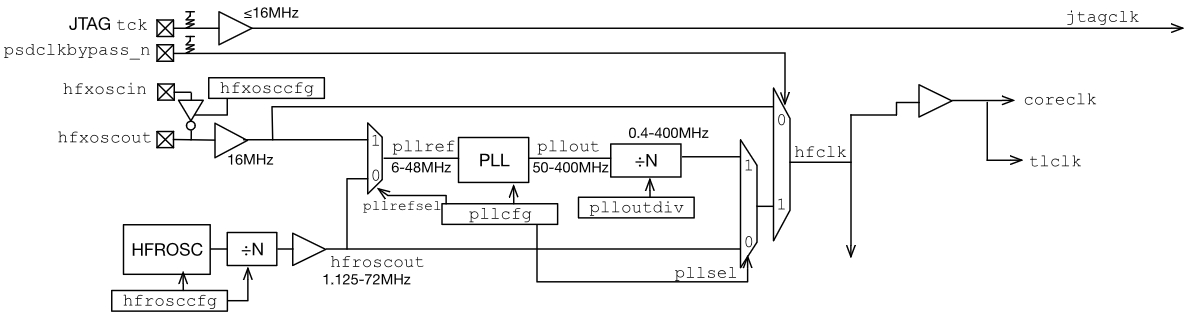
\includegraphics[width=0.9\columnwidth]{figures/hfclock.png}
    \centering
    \caption[High Frequency Clock Diagram]{The high frequency clock generation scheme, specifying how the high frequency clock is driven and configured, taken from the Sifive FE310-G002 Manual\cite{sifive_manual}}
\end{figure}
The high frequency clock controls the processor frequency, and the baud rate of input and output is derived from it. The high frequency clock can be driven from two sources, an internally trimmable high frequency ring oscillator and an external high frequency crystal oscillator. The ring oscillator can produce frequencies ranging form ~1 MHz to 75 MHz, whereas the crystal will produce a constant frequency of 16 MHz. Both of these clock sources may be used `as is', or can be modified using a PLL and divider, giving a available range of 48 MHz to 384 MHz. 
\\
\begin{figure}[H]
    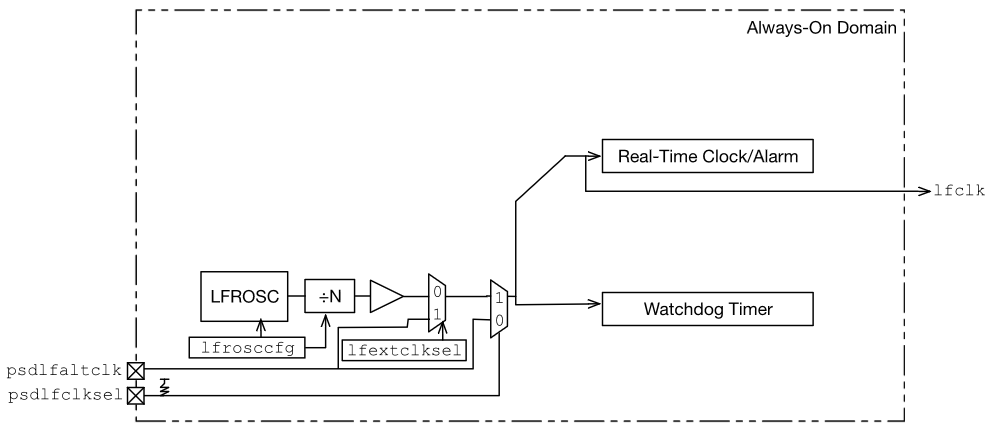
\includegraphics[width=0.9\columnwidth]{figures/lfclock.png}
    \centering
    \caption[Low Frequency Clock Diagram]{The low frequency clock generation scheme, specifying how the low frequency clock is driven and configured\cite{sifive_manual}}
\end{figure}
The low frequency clock is part of the Hifive1 `always on block' and controls the watchdog timer, which can be used to cause a reset on malfunction, and both the real-time clock and the machine timer, both of which are used to generate timed interrupts. Similar to the high frequency clock can be driven from a ring oscillator or from an external clock, which in the Hifive1 is a crystal oscillator. The low frequency ring oscillator functions at 1.5 KHz to 230 KHz using a frequency divider, and the implemented external clock runs at a constant 32.768 KHz, with no option to divide the frequency.
\\
For both clock domains, the crystal oscillator was chosen. The ring oscillator gives the option to operate at a higher frequency, which would result in a higher number of operations per second. While in a practical operating system this would be desirable, since this system is not intended for practical use, a constant frequency was more desirable as it would give more predictable results, and makes \ac{io} operations more reliable. For the low frequency clock, a high frequency would be beneficial for a real time system as the higher frequency would allow for more precise timing of interrupts and other functions, however for an interactive system this precision is not required, and so similar to the high frequency domain the constant frequency of a crystal oscillator was selected.
\subsection{Other Settings}
After the clock has been set up, various other parts of the system also require a one time configuration, ranging from the trap vector to \ac{io} settings.
\section{Traps}
\subsection{Configuration}
When an enabled trap is raised, the pc is set to the trap vector according to the trap mode. The trap vector and mode are stored in the 32 bit csr mtvec. In this csr, bits [1:0] are used to store the mode, where 0 is direct mode and 1 is vectored mode. Bits [31:2] represent vector base address, which is the top 30 bits of a 32 bit address. Since this is stored as 30 bits, two zeros are added to pad the value. This means that the trap handler address must be aligned to 64 bytes. When in direct mode, a trap will set the pc to the base vector address, whereas in vectored mode only synchronous traps are set to the base address, and asynchronous traps set the pc to the base address added to four times the trap code. For this system the vectored mode was chosen. This was because the asynchronous traps are more frequent than synchronous traps, and by jumping to the specific trap call directly a large amount of overhead is skipped. This is relevant for functions like the preemptive scheduler, as it reduces the time to switch processes, which will allow the preemter to be more affective with short quantums.
\subsection{Asynchronous Traps}
Due the use of vectored trap mode, instead of having one single handler for asynchronous traps, each interrupt has it's own handler. Since the Hifive1 does not implement a supervisor mode, there are only 3 available interrupt types, software, timer and external. The software interrupts are not used, as they are mainly used for communication between harts, and the Hifive1 only has a single hart. The machine timer is used for the preemptive scheduler, which will be explored in detail in further sections. Finally the external interrupts, the handler will read from the \ac{clint} claim/complete register. This will provide the handler with the highest priority interrupt code, which will then be used in a jump table to execute the correct interrupt, and once completed the same value is written back to the claim/complete register to indicate that the interrupt has been handled. The interrupts implemented in this will be explored in further sections.
\subsection{Synchronous Traps}
The trap code for syncronous traps can be fetched from the mcause register. This can then be used with a jump table to handle the correct trap.
\section{Processes}
\subsection{Process Structure}
Due to the extremely limited amount of memory available on the Hifive1, the data required to store information on each process has to be structured carefully, else the amount of memory required to store process information would begin to limit the amount of memory available to the processes themselves. In the current implementation, 35 bytes are used to store process information.
\\
One byte each is allocated for a process id, process parent id, process status, and size of a processes text section. For process id and process parent id, only one byte is needed as the Hifive1 does not have the memory to support a large of processes, so a theoretical cap of 256 processes is acceptable. Process status can only take 4 values, so only 2 bits of the byte are used, and the text size byte stores the size as a power of 2, where a process has \(2^n\) words, where \(n\) is the value stored. The mininum number of bits needed to store these is 13, however this would need to be padded to either 32 bits, to ensure that the structure remained word aligned, as an attempt to use the load word instruction on a non word aligned address causes a load address missaligned error. Instead each entry is stored as a byte, as this is the smallest size load that \gls{riscv} allows, which avoids the need to use bit masks to retieve these entries.
\\
One word each is allocated for the processes program counter, text section pointer and address space pointer. Since memory addresses are word length, these cannot be reduced.
\\
The vast majority of the process structure is used storing the 31 general purpose registers. This is required to retain the state of each process in between scheduling. The only option to reduce this would be to limit the amount of registers available to use. Only 31 must be stored as the x0 register is hardwired to zero.
\\
In other systems, information like the processes stack pointer may be stored, however standard RISC-V calling convention specifies x2 to be used as the stack pointer, so separate storing of this information is not required, and allows a process to handle its address space on its own, however on process creation x2 and x3 are initialized as the stack pointer and the global pointer, where the stack pointer points to the bottom of the process address space and the global pointer at the top. This is done to reduce the overhead of processes that use the standard calling convention.
\subsection{States}
% include figure of finite state machine, with running, ready and blocked
Each process has a state, which indicates how the process should be scheduled. In our model, there are four states that a process can be in, ready, running, blocked, and terminated. Running indicates that the process is currently being exectuted. A running process can transition to ready if the scheduler preempts the process, or if the process yields to the processor with an enviroment call. A process will transition to blocked when it makes an interrupt driven \ac{io} call. The blocked process may then transition to ready when the interrupt has been handled. The transition between ready and running is handled by the scheduler, whereas the status of blocked processes are dealt with by each \ac{io} handler. The state value stored in each process entry is used as metadata only except for the terminated state, as instead the scheduler and each \ac{io} handler tracks state by how each process is stored, for instance any process in a queue to be ran is in the ready state, the current process is in the running state, and any processes not in the queue and not running must be blocked. The terminated state indicates to the scheduler that the process should not be requeued.
\section{Scheduler}
This system will be implemented with an interactive scheduler. The functions that the scheduler must perform are storing all the processes that are in the ready state, running ready processes, and preempting processes that have been running for longer than the \gls{quantum}.
\subsection{Creating a Process}
On boot, a table of 7 process entries is allocated in memory, and parts of each are initialized, such as each processes address space and their stack and global pointers. The scheduler will then store the pointer to each entry on a stack, which is used to distribute a process entry to each new process. When a new process is created, the pointer on the top of the stack is used to populate that entry with information about the new process, including the start of the text section which is also used as the processes initial pc, the size of the text section, and the process is also given a sequentially generated process id. Once the process is initialized, it is then added to a queue in the scheduler, which is implemented as a circular queue.
\subsection{Running a process}
To make a process run, the scheduler will first dequeue from the ready processes queue. This will then be used to set the processes state. The stored pc will be used to set the MEPC csr, which stores the value of the pc to return to when mret is called. The \ac{pmp} is then set to allow access to that processes address space, as well as allowing read access to that process text section in the flash memory. The state of the process in the process entry is changed to running. Then most of the registers have their values set, except for t1-4. This is because before these values are set, the sheduler sets the quantum for the process by setting the timer comparison to the current time plus the quantum, and this requires a mininum of 4 registers to to. This is done as close to the start of execution instead of before the registers have their state set, as this ensures the time allowed for each process is as close to the specified quantum as possible. Finally the last 4 registers are set and MRET is called, which begins the execution of the process. The operations of 
\subsection{Preemption}
Each process is given 500 milliseconds of execution time. This time includes execution of user code as well as enviroment calls, however a process cannot be preempted in the middle of an environment call, so if a process reaches the end of its execution time during an environment call, it will be preempted as soon as the system returns to the user code. As previously mentioned, the preemption is timed using the machine timer interrupts. The machine timer was chosen over the timer interrupt generated by the AON unit, as the latter interrupt is part of the external interrupts so there is an increased amount of overhead required for it to be processed. Using the machine timer interrupt also addresses another problem, which is maintaining the state of the process. When the preemption occurs, the first thing that must happen is that the processes registers must be saved to the process entry, which requires the global pointer. The global pointer is a constant value, as it always points to top of the machine address space, however to use it, it must be stored into a register, which requires that registers value to be store to the machine stack. For this we use the mscratch csr to store the machine pointer during normal execution, which when in machine mode we swap with the current processes stack pointer. This allows us to use the machine stack while also storing the processes stack. In addition to the global pointer we also save the value in t0 and t1 to store the process entry pointer, and to pop and store the values back from the stack and the mscratch csr, before saving each of the remaining 26 registers. The operations of the preempter occur as follows:
\begin{enumerate}
    \item The \ac{pmp} is reset, clearing all user memory access
    \item The fence.i instruction is called, which invalidates all entries in the instuction cache
    \item The process sp is switched with the machine sp in the mscratch csr
    \item Registers gp, t0, and t1 are pushed to the stack
    \item The global pointer is loaded into gp, and used to load the current process entry pointer into t0
    \item The 3 values pushed to the stack are each pop into t1 and then stored into the process entry, as well the the value that was swapped into the mscratch csr
    \item All 26 remaining registers are stored to the process entry
    \item The value stored in the mepc csr is loaded and stored
    \item If the process had the running state, it is changed to ready, otherwise it remains unchanged.
    \item If the status is terminated, add the process entry pointer to the free entry stack
    \item Else add the pointer to the process queue
\end{enumerate}
\section{Memory Management}
% figures, diagram of memory split into address spaces, labeled process 0 to 6 and machine memory

\section{IO}